\chapter{Reference}
\label{Reference}
\typeout{$Id$}

\section{Main Window}
\label{Main}

\begin{figure}[hbpt]
\begin{centering}
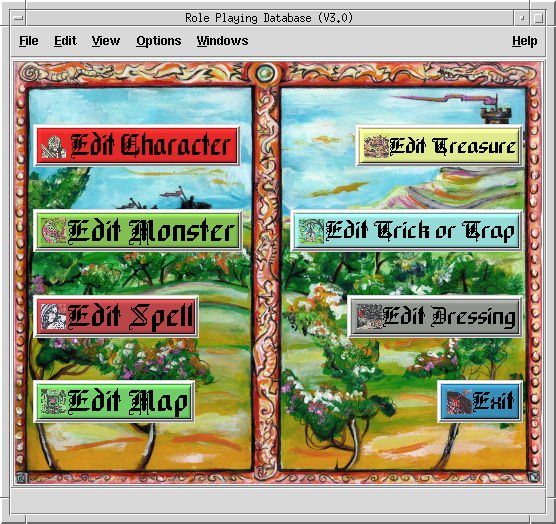
\includegraphics[width=5in]{MainWindow.png}
\caption{The main window of the Role Playing Database}
\label{fig:main}
\end{centering}
\end{figure}
The main window, shown in Figure~\ref{fig:main}, contains buttons for
the seven game informational editors: Character, Monster, Spell,
Treasure, Trick / Trap, Map, and Dressing.  An eighth button selects
for program exit. In addition to the eight buttons, there are drop down
menus on a menu bar.  The same menu bar is used on all of the major
top-level screens.  The File menu has the standard New, Open, Save,
Save As, Print, Close, and Exit menu items, all of which have the
expected meanings and functionallity.  The New and Open menu items on
the File menu use cascading menus to select the sort of thing to create
or open.  The Options menu contains menu items to create/edit, read,
and write the program's main coniguation file, plus a menu item to edit
template files, which are created and maintaine the ``Sheet Template
Editor'' windom (See Section~\ref{Template}).  The Windows menu
contains menu items to select one of the existing toplevel windows. The
Help menu provides access to the online help system (see
Chapter~\ref{Help} for complete information about using the on-line help).

\section{Sheet Template Editor Window}
\label{Template}

\begin{figure}[hbpt]
\begin{centering}
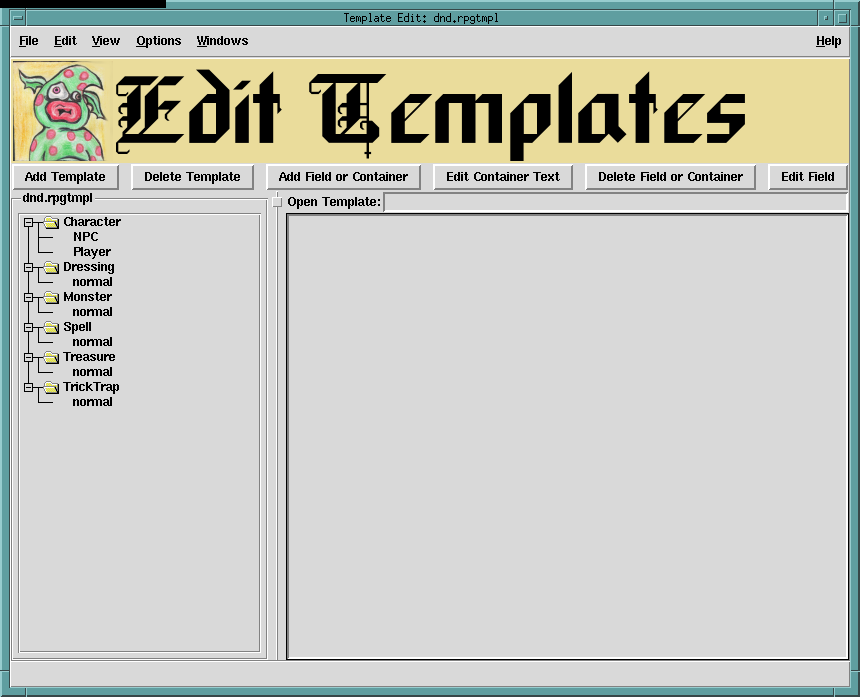
\includegraphics[width=5in]{TemplateEditor1.png}
\caption{The initial Template Editor Window}
\label{fig:tmped1}
\end{centering}
\end{figure}
\begin{figure}[hbpt]
\begin{centering}
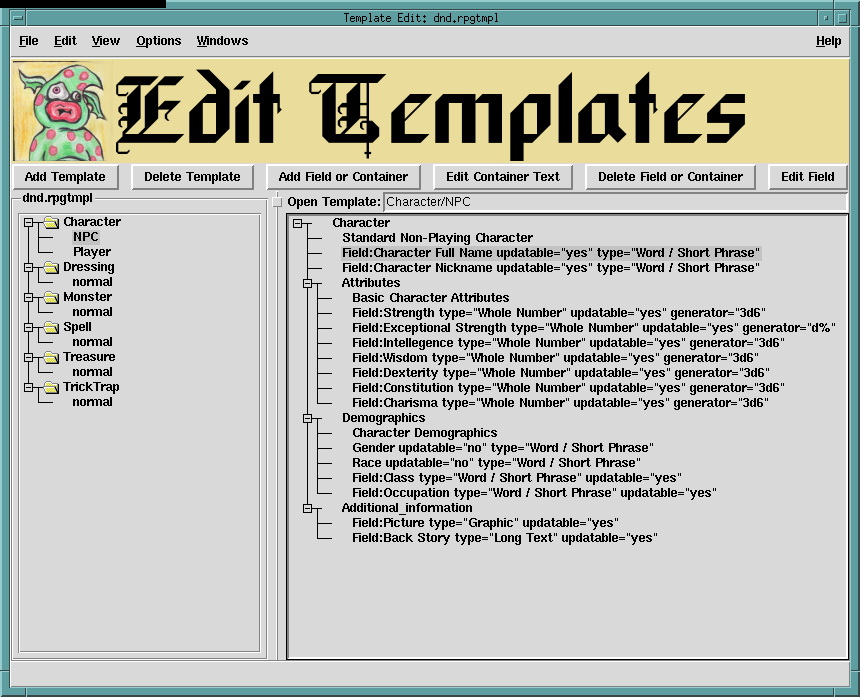
\includegraphics[width=5in]{TemplateEditor2.png}
\caption{The Template Editor Window after loading a template}
\label{fig:tmped2}
\end{centering}
\end{figure}
To allow for differences in game systems, game data elements are
defined with the use of templates.  These templates define what
information is recorded for each game element for a given game system. 
These templates are created and maintained with the template editor. 
The template editor in invoked from the Options menu.  The editor is
shown in Figures~\ref{fig:tmped1} and \ref{fig:tmped2}.  A sheet
contains a toplevel container which in turn contains zero or more fields
or containers.  Containers can contains zero or more fields or
containers.  Fields and containers have names. Fields also have a type,
possibly a generator (dice combination), and a flag that indicates whether the
field value can be updated.  There are five defined field types:

\begin{enumerate}
\item \verb=Whole Number=--This is a numerically valued field. It is either
an arbitary (usually fixed) value or the result of a dice throw.
\item \verb=Word / Short Phrase=--This either a single word or a short
(one line at most) phrase, generally describing a textual attribute,
such as a name or some sort of descriptive condition or status.
\item \verb=Long Text=--This is a multi-line, but short (1-2 paragraph)
description text value.
\item \verb=Graphic=--This is a picture file\footnote{The graphic file
is copied into the sheet file and remains part of the sheet file object.}.
\item \verb=Document=--This a document file\footnote{The document file
is copied into the sheet file and also remains part of the sheet file
object.}.
\end{enumerate}

The generator attribute is only used for numerically valued fields and
the updatable attribute can only be set to no for the word / short
phrase and numerically valued fields.

The templates are used for Character, Monster, Spell, Treasure, Trick /
Trap, and Dressing sheet editors.  The Map editor uses a set of hard-coded
templates. These templates define the fields, their attributes, and
grouping / organiational structure.  Containers have a text attribute
that is used as a section heading for the group of fields contained in
the container. The included template file, \verb=dnd.rpgtmpl=, defines
informational sheets suitable for \textit{Advanced Dungeons and
Dragons}, but template files for other game systems can be created.

\section{Character Editing Window}
\label{Character}

\begin{figure}[hbpt]
\begin{centering}
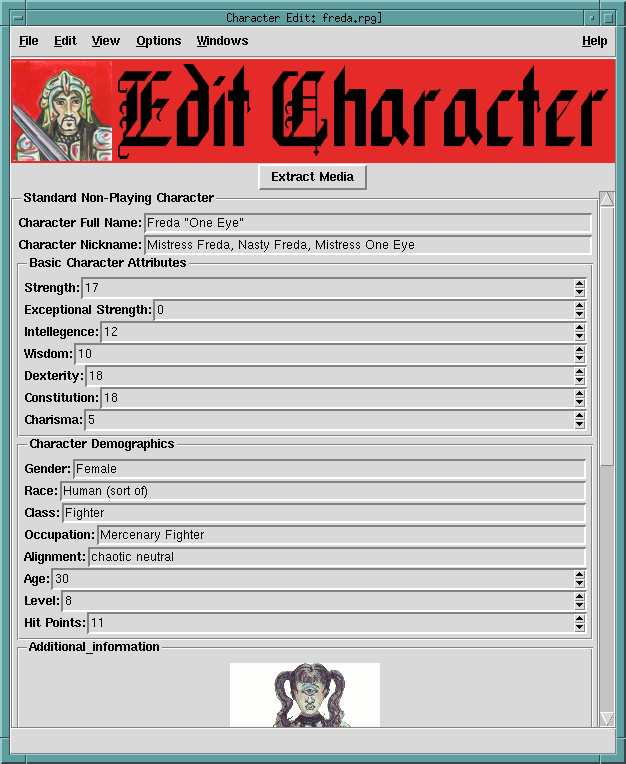
\includegraphics[width=5in]{CharacterEditor.png}
\caption{The Character Editor window of the Role Playing Database}
\label{fig:char}
\end{centering}
\end{figure}
The Character Editing Window, shown in Figure~\ref{fig:char}, is used to
edit characters, both playing and non-playing characters.  It uses one
of the Character templates defined in the current template file.

\section{Monster Editing Window}
\label{Monster}

\section{Spell Editing Window}
\label{Spell}

\section{Treasure Editing Window}
\label{Treasure}

\section{Trick / Trap Editing Window}
\label{TrickTrap}

\section{Dressing Editing Window}
\label{Dressing}

\section{Map Editing Window}
\label{Map}


